\subsection{Vertical diffusion and junction formation (Well formation)}\label{building_wells}
The goal of most diffusions is to form pn junctions by converting p-type material to n-type material or vice versa.
In \autoref{junction_formation_plot}, for example, the wafer is uniformly doped n-type material with a concentration indicated by $N_B$, and the diffusing impurity is boron.
The point at which the diffused impurity profile intersects the background concentration is the mettalurgical junction depth ($x_j$).
The net impurity concentration at $x_j$ is zero.
Setting $N(x)$ equal to the background concentration $N_B$ at $x=x_j$ yields\footnote{Gerold W. Neudeck and Robert F. Pierret, Modular series on solid state devices, Volume V, Chapter 4}
\begin{equation}
x_j
=
2 \cdot\sqrt{D \cdot t \cdot \ln\left(\frac{N_0}{N_B}\right)}
\end{equation}
and
\begin{equation}
x_j
=
2 \cdot\sqrt{D \cdot t}
\cdot
\erfc^{-1}\left(\frac{N_B}{N_0}\right)
\end{equation}

for the Gaussian and complementary error function distributions, respectively.

In \autoref{junction_formation_plot}, the boron concentration $N$ exceeds $N_B$ to the left of the junction, and this region is p-type.
To the right of $x_j$, $N$ is less than $N_B$, and this region remains n-type.

To calculate the junction depth, we must know the background concentration $N_B$ of the original wafer.
Look at \autoref{r_l_nd_relation} for this purpose.

\begin{figure}[H]
	\centering
	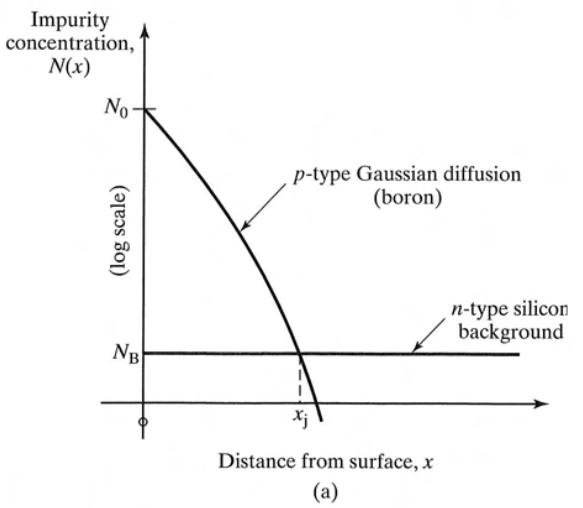
\includegraphics[scale=0.5]{well_formation1.png}
	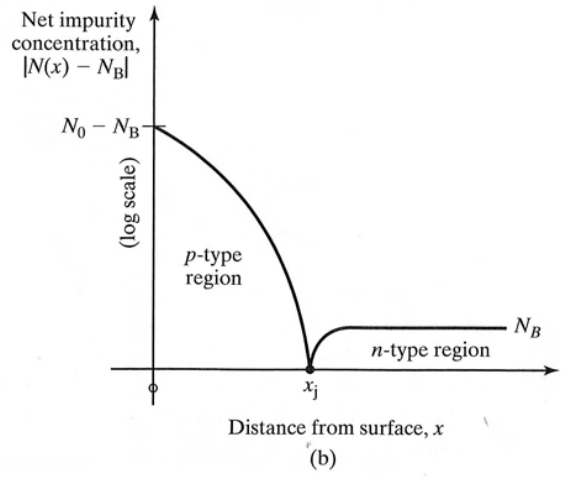
\includegraphics[scale=0.5]{well_formation2.png}
	\caption{Formation of a pn junction by diffusion: (a) An example of a p-type Gaussian diffusion into a uniformly doped n-type wafer; (b) net impurity concentration in the wafer.}
	\label{junction_formation_plot}
\end{figure}

